\subsubsection{Introduction}
According to \citep{buss2004introduction,barinka2002inverse} there are several methods to solve the inverse kinematics problem. For this part I decided to analyse other approach of solving this problem. The method I decided to evaluate was an iterative method using the pseudo inverse of the Jacobian matrix, similar to the one used in \citep{bhatti2014forward}.

\begin{equation}
x=f(\theta)
\end{equation}

\subsubsection{Iterative model}
The idea behind this method is that by performing a change in the joint space will bring as a consequence  change in the Cartesian space, this is described by forward kinematics. Therefore if the current configuration is known it is possible to compute the position of the end effector and if the desired position is very close to current position only a slight change in the configuration is needed to achieve that desired position.

\begin{equation}
\label{eq:part3.jacobian_relation}
dx=J(\theta)d\theta
\end{equation}

The relationship between a small change in the joint space and the change in the Cartesian space is given  by (\ref{eq:part3.jacobian_relation}), where $J(\theta)$ is the Jacobian matrix that is defined as:

\begin{equation}
J(\theta)=  \left[
\begin{array}{ccc}
	\frac{\partial f_1}{\partial x_1} & \cdots & \frac{\partial f_1}{\partial x_n} \\
	\vdots & \ddots & \vdots \\
	\frac{\partial f_m}{\partial x_1} & \cdots & \frac{\partial f_m}{\partial x_n} \\
\end{array}
\right] 
\end{equation}

As a consequence, the inverse kinematics problem can be solved by knowing the difference between the current configuration and the configuration that arrives to de desired position, let name it $\Delta\theta$.

\begin{equation}
\theta_d=\theta+\Delta\theta
\end{equation}

If $\Delta\theta$ is considered to be small it can be computed by using inverse Jacobian as expressed in (\ref{eq:part3.delta_relation}). Usually as the inverse of Jacobian matrix not always exists, it is necessary to use the pseudo-inverse as denoted by \citep{penrose1955generalized}.

\begin{equation}
\label{eq:part3.delta_relation}
\Delta\theta \approx  J(\theta)^{*}\Delta x
\end{equation}

where $J(\theta)^{*}$ is the pseudo-inverse and is computed using (\ref{eq:part3.pseudo_inverse}). The value of $\Delta x$ is the difference or the error between the current position and the desired position 

\begin{equation}
\label{eq:part3.pseudo_inverse}
J(\theta)^{*} = J(\theta)^T(J(\theta)J(\theta)^T)^-1
\end{equation}

Furthermore, a step factor can be added to the equation and completely get the joint values that reduces error and get closer to the desired position.

\begin{equation}
\begin{aligned}
\theta & = \theta + \alpha\Delta\theta \\
& = \theta + \alpha J(\theta)^{*}e \\
&=  \theta + \alpha J(\theta)^{*}(\theta_d - \theta)
\end{aligned}
\end{equation}

Finally, the current joint values are updated using small steps, controlled by $\alpha$, until the error is zero or very close to zero, where can present oscillations  due to the value of $\alpha$ and the precision of the robot.

\subsubsection{Simulation and results}
For the simulation it was considered a planar robot with two revolute joints, with links of length $a_1=20 [cm]$ and $a_2=10 [cm]$, the coefficient $\alpha = 0.1$. The Jacobian of the robot is:

\begin{equation}
J(\theta) = \left[ \begin{array}{cc}
	-a_1\sin(q_1) - a_2\sin(q_1+q_2) & -a_2\sin(q_1+q_2) \\
        a_1\cos(q_1)+a_2\cos(q_1+q_2) & a_2\cos(q_1+q_2) \\
\end{array} \right] 
\end{equation}

The experiment consists of propose the value of a point in the configuration space $Q_d=[ \begin{array}{cc} q_{d1} & q_{d2} \\ \end{array} ]^T$ and perform forward kinematics to get the point $P_d \in R^3$, then repeat the process but using a new random point in the configuration space which will lead to a different position in the Cartesian space that will represent the current position, $Pd \neq P$. Therefore the magnitude of error in the Cartesian space will be greater that zero $||e|| > 0$.

\begin{figure}[htbp] 
\begin{center}
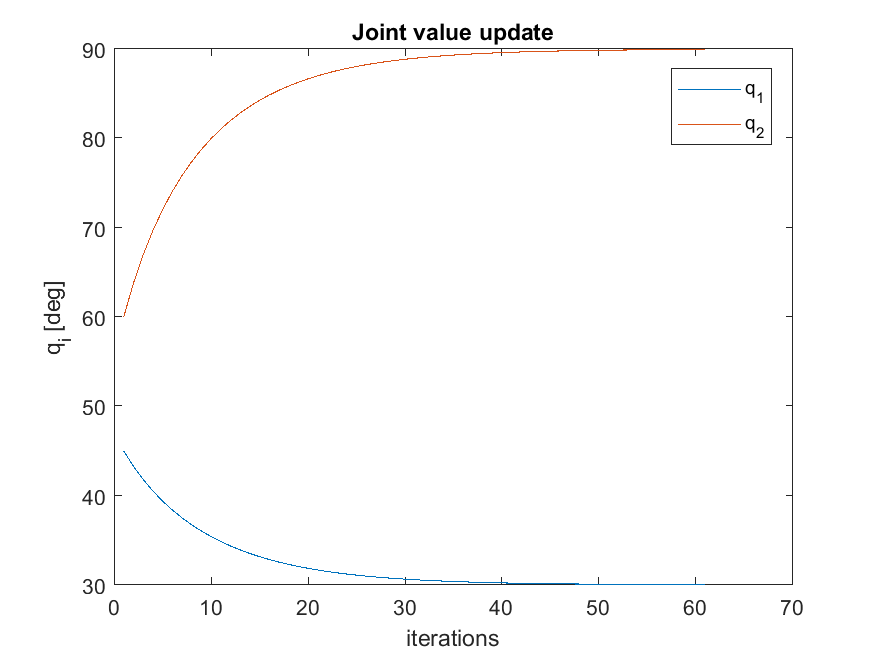
\includegraphics[width=\textwidth]{images/Trajectory_Joint_p3_rodrigo}
\caption{Update process of joint values over the iterations of using the iterative method}
\label{fig:part3.joint_trajectory}
\end{center}
\end{figure}

As the problem is to find the values in joint space that achieves the desired point in Cartesian space, the iterative method is used and for every iteration the joint values converge to the solution, depicted in figure \ref{fig:part3.joint_trajectory}. Moreover, after the joint values are updated the forward kinematics is performed again and the error is also updated and minimised, as depicted in figure \ref{fig:part3.error_minimisation}.

The code \ref{apendix:iterative_method}

\begin{figure}[htbp] 
\begin{center}
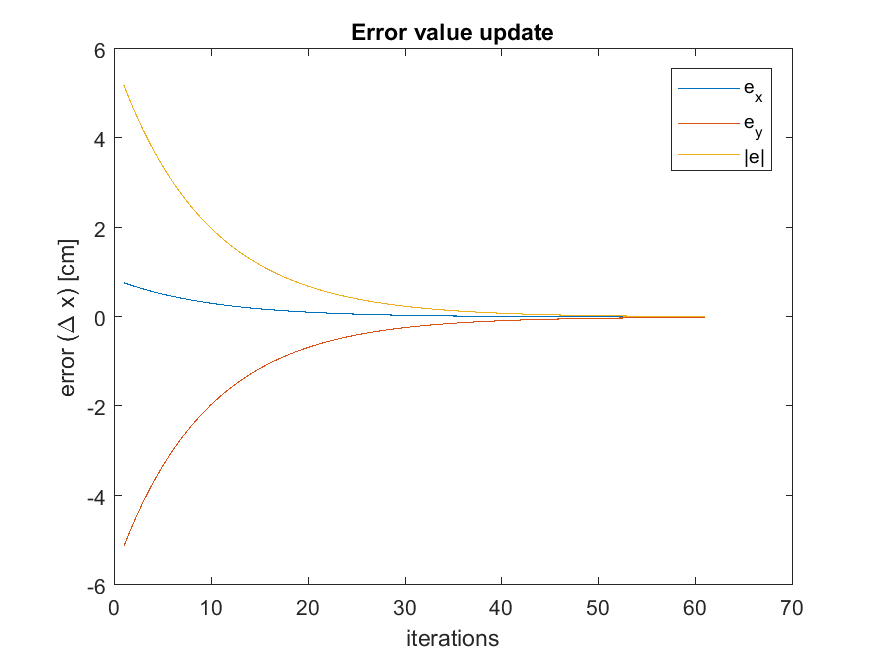
\includegraphics[width=\textwidth]{images/error_p3_rodrigo}
\caption{Error is minimised as the position of end effector gets closer to the desired position}
\label{fig:part3.error_minimisation}
\end{center}
\end{figure}